% ============================================================
% M3 S3 练习件·W2 臂C —— 课时15 2.7.1抛物线方程（照课时01母版体例件）
% 生成：M3 成卷轮 S3 W2 臂C｜2026-09-14｜编译 cwd＝本目录（中文路径禁 \input 绝对路径）
%   xelatex main-true.tex ×2 → 含详解印本；xelatex main-false.tex ×2 → 纯题版（单源双本）
% 输入链（全只读）：题面库 课时15-2.7.1抛物线方程.md（题面逐字装配）＋ -答案侧.md（值逐字回嵌）
%   ＋ 定稿/批D-课时15-2.7.1抛物线方程.md（详解回嵌源＝§7.1 补产全文）；toolchain＝qp-m3.sty
%   （钉后版 md5 7c3930362be8a0a2bdf21bbf8ac16573，本地挂载副本，破损即停）。
% 母版体例：详见 课时01《练习件母版体例说明.md》；门谱读数见 工作区/_tmpM3S3W2臂C0914/。
% 键账：件内 ansblock 键集 ≡ 题面库片练键集 ≡ manifest 练键序 2章-练-课时15-01~16（16 键，
%   零缺漏零多余）；拓区隔离：2章-拓/测/滚 键不入本件（S4 拓展册收）；导学键 G1~G5 属导学件域，亦不入。
% 卷式例外案B：练习件不属卷式——答案块物理落点恒为题后 ansblock，禁卷末附卷制；
%   全线括线模（导言 \ansblockgrayfalse 一次置定，件内不切换；灰底盒不可跨栏断，练习件禁用）。
% 题序＝manifest 键序 01~16（零重排）；印面题号 1~16 连号（\tihao 号＝\ansitem 号同键）；
%   三档切位 1~7／8~14／15~16（照库序切位，非难度重排；15~16＝0.40/0.65 难档压轴对）。
% 槽配实录：单选2（题5/13）＋填空5（题2/3/4/11/12）＋解答9（余）；多选 0（manifest 期望值多选数＝0）；
%   本片实配照题面侧头标（批D §四 满足度表同口径）。
% 选项槽位：默认四连排（0.25\linewidth−0.25\lxhang），超宽降档梯 四连排→两连排
%   （0.5\linewidth−0.5\lxhang−0.25em）→单列 \lxopt；禁缩字号/负 kern/删标点凑宽。
%   本片实测降档（槽宽门读数 0914）：题5 两连排（strict 预警 C槽「抛物线」47.2pt＞85%线46.2pt，
%   占四连排槽 87%）；题13 保持四连排（zero-fp/strict 双档全过）。
% 解答书写区：解答9题逐题 \liubai（题7/15 两小问 24mm；余无小问 16mm；cap 40mm 带内；
%   纯题档吞 ansblock 不吞 \liubai）。
% 填空印答：题2/3/4/11/12 空位 \kongda{值}（详解版印答、纯题版退定宽空线，两档等形；
%   题12 双空拆两空位）；空位标点照库逐字留空位外。
% tieside：难度×知识点承导学件同源 例/变 槽标签（底稿回核预排，逐题登记见值台账；
%   题14＝变4 中档(知识点一) 系源签例外随源；导学件异动按变更协议回核）。
% 详解源注：16 题详解全承 S2 导学件同源宏文（映射 例1/变6/变2/例13/例3/变18/例7/变12/
%   变14/例19/例15/变20/变22/变4/例31/例23；ansitem 值与答案侧字节一致，ansnote 单物理行）；
%   详解句末标点照批D 定稿回改（．→。；小数点 2.25/4.5 等照旧）。
% 印面清洗：题面侧【注】行不入印面；题1/题13 题面 ASCII 引号宏化 CJK 弯引号（照课时10 先例）；
%   题13「如图1/图2」装饰图不回补（裁定免图销案，文字自足）；题16 图注尺寸经 0914 印前
%   回冲为真图（图资源/15-16.png，\ansfig 插桩，图注括注随真图摘除；台账「图债」同账）。
% ============================================================
\documentclass[fontset=none]{ctexart}
\usepackage{qp-m3}
% —— 印面逐字符号路由补钉（承导学件母版；− 走 TNR、▱ NSC 子块；禁改 sty 保 md5） ——
\xeCJKDeclareCharClass{Default}{"2212}%
\setCJKfamilyfont{nscblk}[Path=C:/提示词/工作区/字替对照-0909/variantF/fonts/,BoldFont=NSC-w600.ttf]{NSC-w500.ttf}%
\xeCJKDeclareSubCJKBlock{nscblk}{"25B1}%
\newcommand{\pxparallelogram}{{\CJKfamily{nscblk}▱}}%
% —— 断行微调（承导学件母版实测档，三零门承重；\emergencystretch 不另设） ——
\xeCJKsetup{CJKglue={\hskip 0.10em plus 0.08em minus 0.05em}}%
% —— 练习件全线括线模（S3 波次方案 §四.3：导言一次置定、件内不切换） ——
\ansblockgrayfalse
% —— 页脚件名（qp-headfoot 复用入口） ——
\renewcommand{\qpzhangming}{第二章\quad 平面解析几何}%
\renewcommand{\qpjianming}{练习件}%

\begin{document}

\keshi{第15课时\quad 抛物线的标准方程}
\begin{multicols}{2}
\emergencystretch=1em

% ============================================================
% 基础巩固（题1~7＝练01~07：解答4＋单选1＋填空2，照库序切位；题后紧跟答案制，全线括线 ansblock）
% ============================================================
\dangbadge{基}{础}{巩}{固}

\tihao{1}\zu{抛物线定义辨析×解答} \tieside{简单(知识点一)}【微思考】在抛物线定义中，若去掉条件“\(l\)不经过点\(F\)”，点的轨迹还是抛物线吗？
\liubai[16mm]{解答书写区}

\begin{ansblock}[2章-练-课时15-01]
% ans:2章-练-课时15-01
\ansitem{1}{不是。当定点 F 在直线 l 上时，动点轨迹是与 l 垂直的直线（过 F）。}
\ansnote{详解}{取\(l\)为\(x\)轴、\(F\)为原点。动点\(P(x,y)\)到\(F\)的距离为\(\sqrt{x^{2}+y^{2}}\)，到\(l\)的距离为\(|y|\)。\par\noindent “到\(F\)与到\(l\)距离相等”：\(\sqrt{x^{2}+y^{2}}=|y|\)，平方得\(x^{2}+y^{2}=y^{2}\)，即\(x=0\)。轨迹为整条\(y\)轴：过\(F\)且垂直于\(l\)的直线，不是抛物线（\(p=0\)时抛物线无意义）。验算：点\((0,5)\)到\(F\)距离5、到\(x\)轴距离5，相等合。}
\end{ansblock}

\tihao{2}\zu{焦准距与四种标准方程×填空} \tieside{简单(知识点二)}焦点到准线的距离为\(3/2\)的抛物线的标准方程为\kongda{y²=3x 或 y²=−3x 或 x²=3y 或 x²=−3y}。

\begin{ansblock}[2章-练-课时15-02]
% ans:2章-练-课时15-02
\ansitem{2}{y²=3x 或 y²=−3x 或 x²=3y 或 x²=−3y。}
\ansnote{详解}{焦准距即\(p\)：\(p=3/2\)，\(2p=3\)。开口未指定，四种标准方程并立：\(y^{2}=3x\)、\(y^{2}=-3x\)、\(x^{2}=3y\)、\(x^{2}=-3y\)。}
\end{ansblock}

\tihao{3}\zu{焦准距与四种标准方程×填空} \tieside{简单(知识点一)}与点\(F(0,-3)\)和直线\(y-3=0\)的距离相等的点的轨迹方程是\kongda{x²=−12y}。

\begin{ansblock}[2章-练-课时15-03]
% ans:2章-练-课时15-03
\ansitem{3}{x²=−12y}
\ansnote{详解}{\(F(0,-3)\)不在直线\(y=3\)上，由定义轨迹为抛物线：焦点\(F(0,-3)\)，准线\(y=3\)。开口向下，设\(x^{2}=-2py\)（\(p>0\)）：\(p/2=3\)，\(p=6\)，方程\(x^{2}=-12y\)。验算：顶点\((0,0)\)到\(F\)距3、到准线距3合。}
\end{ansblock}

\tihao{4}\zu{依点求方程×填空} \tieside{简单(知识点二)}顶点在原点，焦点在\(x\)轴上，且过点\((-4,-8)\)的抛物线方程为\kongda{y²=−16x}。

\begin{ansblock}[2章-练-课时15-04]
% ans:2章-练-课时15-04
\ansitem{4}{y²=−16x}
\ansnote{详解}{焦点在\(x\)轴，设\(y^{2}=mx\)（\(m\neq 0\)）。代入\((-4,-8)\)：\(64=m\times (-4)\)，\(m=-16\)，方程\(y^{2}=-16x\)（开口向左，与横坐标为负相符）。}
\end{ansblock}

\tihao{5}\zu{定义式识别轨迹×单选} \tieside{简单(知识点一)}已知实数\(x\)，\(y\)满足\(\sqrt{x^{2}+(y-p/2)^{2}}=|y+p/2|\)，其中常数\(p>0\)，则动点\(P(x,y)\)的轨迹是\nobreak(\kongwei)
\bindopt {\fontsize{10.5pt}{\qpTJgLeadLiti}\selectfont \makebox[\dimexpr0.5\linewidth-0.5\lxhang-0.25em\relax][l]{A．射线}\makebox[\dimexpr0.5\linewidth-0.5\lxhang-0.25em\relax][l]{B．直线}\par}
\bindopt {\fontsize{10.5pt}{\qpTJgLeadLiti}\selectfont \makebox[\dimexpr0.5\linewidth-0.5\lxhang-0.25em\relax][l]{C．抛物线}\makebox[\dimexpr0.5\linewidth-0.5\lxhang-0.25em\relax][l]{D．椭圆}\par}

\begin{ansblock}[2章-练-课时15-05]
% ans:2章-练-课时15-05
\ansitem{5}{C}
\ansnote{详解}{左端为\(P(x,y)\)到定点\(F(0,p/2)\)的距离；右端\(|y+p/2|\)为\(P\)到定直线\(l\)：\(y=-p/2\)的距离。\(F(0,p/2)\)不在\(l\)上（\(p>0\)），由抛物线定义，轨迹为抛物线，故选C。}
\end{ansblock}

\tihao{6}\zu{焦半径与定义互化×解答} \tieside{简单(知识点三)}已知\(M\)是抛物线上一点，且\(M\)到抛物线的焦点的距离等于3，写出\(M\)到抛物线的准线的距离．
\liubai[16mm]{解答书写区}

\begin{ansblock}[2章-练-课时15-06]
% ans:2章-练-课时15-06
\ansitem{6}{3}
\ansnote{详解}{由抛物线定义，抛物线上点到焦点的距离与到准线的距离相等，故\(M\)到准线的距离为\(|MF|=3\)。}
\end{ansblock}

\tihao{7}\zu{焦准距与四种标准方程×解答} \tieside{简单(知识点二)}分别根据下列条件，写出抛物线的标准方程：
(1) 焦点是\(F(2,0)\)；(2) 准线方程是\(x=-3/2\)．
\liubai[24mm]{解答书写区}

\begin{ansblock}[2章-练-课时15-07]
% ans:2章-练-课时15-07
\ansitem{7}{(1) y²=8x；(2) y²=6x。}
\ansnote{详解}{(1)焦点\((2,0)\)在\(x\)正半轴：\(p/2=2\)，\(p=4\)，\(2p=8\)，方程\(y^{2}=8x\)。(2)准线\(x=-3/2\)得焦点在\(x\)正半轴：\(p/2=3/2\)，\(p=3\)，\(2p=6\)，方程\(y^{2}=6x\)。验算：(1)准线\(x=-2\)合；(2)焦点\((3/2,0)\)合。}
\end{ansblock}

\tihao{8}\zu{依点求方程×解答} \tieside{简单(知识点二)}已知抛物线的焦点在\(x\)轴的正半轴上，且准线与\(y\)轴之间的距离为6，求此抛物线的标准方程．
\liubai[16mm]{解答书写区}

\begin{ansblock}[2章-练-课时15-08]
% ans:2章-练-课时15-08
\ansitem{8}{y²=24x}
\ansnote{详解}{焦点在\(x\)正半轴，开口向右，设\(y^{2}=2px\)（\(p>0\)），准线\(x=-p/2\)。准线与\(y\)轴距离\(|-p/2|=6\)得\(p=12\)，\(2p=24\)，方程\(y^{2}=24x\)。验算：焦点\((6,0)\)、准线\(x=-6\)，与\(y\)轴距离均为6合。}
\end{ansblock}

\tihao{9}\zu{依点求方程×解答} \tieside{简单(知识点二)}求焦点在\(x\)轴正半轴上，并且经过点\(M(2,-4)\)的抛物线的标准方程．
\liubai[16mm]{解答书写区}

\begin{ansblock}[2章-练-课时15-09]
% ans:2章-练-课时15-09
\ansitem{9}{y²=8x}
\ansnote{详解}{设\(y^{2}=2px\)（\(p>0\)）。代入\((2,-4)\)：\(16=4p\)，\(p=4\)，\(2p=8\)，方程\(y^{2}=8x\)。验算：焦点\((2,0)\)、准线\(x=-2\)；\(M(2,-4)\)到焦点距离4、到准线距离4合。}
\end{ansblock}

\tihao{10}\zu{焦半径与定义互化×解答} \tieside{简单(知识点三)}已知点\(M\)在抛物线\(y^{2}=12x\)上，它到焦点的距离等于9，求点\(M\)的坐标．
\liubai[16mm]{解答书写区}

\begin{ansblock}[2章-练-课时15-10]
% ans:2章-练-课时15-10
\ansitem{10}{M(6,6√2) 或 M(6,−6√2)。}
\ansnote{详解}{\(y^{2}=12x\)：\(2p=12\)，\(p=6\)，准线\(x=-3\)。由定义\(|MF|=x_M+3=9\)，得\(x_M=6\)；代入得\(y^{2}=72\)，\(y=\pm 6\sqrt{2}\)。故\(M(6,6\sqrt{2})\)或\(M(6,-6\sqrt{2})\)（两点均在抛物线上，关于\(x\)轴对称）。验算：\(\sqrt{(6-3)^{2}+72}=\sqrt{81}=9\)合。}
\end{ansblock}

\tihao{11}\zu{依点求方程×填空} \tieside{中档(知识点二)}已知抛物线过点\(A(2,-4)\)，则抛物线的标准方程为\kongda{y²=8x 或 x²=−y}．

\begin{ansblock}[2章-练-课时15-11]
% ans:2章-练-课时15-11
\ansitem{11}{y²=8x 或 x²=−y}
\ansnote{详解}{\(A(2,-4)\)在第四象限，开口向右或向下。开口向右：设\(y^{2}=2px\)（\(p>0\)），\((-4)^{2}=2p\times 2\)得\(p=4\)，方程\(y^{2}=8x\)；开口向下：设\(x^{2}=-2py\)（\(p>0\)），\(4=-2p\times (-4)\)得\(p=1/2\)，方程\(x^{2}=-y\)。综上\(y^{2}=8x\)或\(x^{2}=-y\)。验算：\(4^{2}=8\times 2\)合；\(2^{2}=-(-4)\)合。}
\end{ansblock}

\tihao{12}\zu{距离和定值的轨迹×填空} \tieside{中档(知识点三)}已知曲线\(C\)是平面内到定点\(F(0,1)\)和定直线\(l\)：\(y=-1\)的距离之和等于3的动点\(P\)的轨迹，则曲线\(C\)的一条对称轴方程是\kongda{x=0}，\(|PF|\)的最小值是\kongda{1/2}。

\begin{ansblock}[2章-练-课时15-12]
% ans:2章-练-课时15-12
\ansitem{12}{x=0；1/2。}
\ansnote{详解}{设\(P(x,y)\)：\(\sqrt{x^{2}+(y-1)^{2}}+|y+1|=3\)。①\(y>2\)或\(y<-4\)（\(|y+1|>3\)）：左边\(>3\)，无解；②\(-1\leqslant y\leqslant 2\)：\(\sqrt{x^{2}+(y-1)^{2}}=2-y\)，平方得\(x^{2}=-2y+3\)（\(-1\leqslant y\leqslant 3/2\)），对称轴\(x=0\)，此时\(|PF|=2-y\geqslant 1/2\)；\par\noindent ③\(-4\leqslant y<-1\)：\(\sqrt{x^{2}+(y-1)^{2}}=y+4\)，平方得\(x^{2}=10y+15\)（\(-3/2\leqslant y<-1\)），对称轴\(x=0\)，此时\(|PF|=y+4\geqslant 5/2\)。综上，对称轴方程\(x=0\)，\(|PF|_{\min}=1/2\)。验算：②段平方展开\(x^{2}+(y-1)^{2}=(2-y)^{2}\)得\(x^{2}=-2y+3\)合；②段与③段区间衔接经复核无缝合。}
\end{ansblock}

\tihao{13}\zu{实际背景建模求方程×单选} \tieside{中档(知识点三)}苏州市“东方之门”是由两栋超高层建筑组成的双塔连体建筑（如图1所示），“门”的内侧曲线呈抛物线形．图2 是“东方之门”的示意图，已知\(|CD|=30\)m，\(|AB|=60\)m，点\(D\)到直线\(AB\)的距离为 150m，则此抛物线顶端\(O\)到\(AB\)的距离为\nobreak(\kongwei)
\bindopt {\fontsize{10.5pt}{\qpTJgLeadLiti}\selectfont \makebox[\dimexpr0.25\linewidth-0.25\lxhang\relax][l]{A．180m}\makebox[\dimexpr0.25\linewidth-0.25\lxhang\relax][l]{B．200m}\makebox[\dimexpr0.25\linewidth-0.25\lxhang\relax][l]{C．220m}\makebox[\dimexpr0.25\linewidth-0.25\lxhang\relax][l]{D．240m}\par}

\begin{ansblock}[2章-练-课时15-13]
% ans:2章-练-课时15-13
\ansitem{13}{B}
\ansnote{详解}{以顶端\(O\)为原点建系，设\(x^{2}=-2py\)（\(p>0\)）。由对称性\(D(15,h)\)（\(h<0\)），\(B(30,h-150)\)。联立：\(225=-2ph\)，\(900=-2p(h-150)\)。两式相除：\(4=(h-150)/h\)，得\(h=-50\)；代入\(225=-2p\times (-50)\)得\(p=2.25\)。顶端\(O\)到\(AB\)的距离\(=|h|+150=200\)(m)，故选B。验算：\(p=2.25\)，\(2p=4.5\)，\(900=4.5\times 200\)合。}
\end{ansblock}

\tihao{14}\zu{定义退化与分类轨迹×解答} \tieside{中档(知识点一)}已知点\(M\)到点\(F(4,0)\)的距离比它到直线\(l\)：\(x+6=0\)的距离小2，求点\(M\)的轨迹方程．
\liubai[16mm]{解答书写区}

\begin{ansblock}[2章-练-课时15-14]
% ans:2章-练-课时15-14
\ansitem{14}{y²=16x。}
\ansnote{详解}{设\(M(x,y)\)。“\(|MF|\)比到\(l\)的距离小2”即\(|x+6|-|MF|=2\)。当\(x\geqslant -6\)时：\(x+6-\sqrt{(x-4)^{2}+y^{2}}=2\)，即\(\sqrt{(x-4)^{2}+y^{2}}=x+4\)（隐含\(x\geqslant -4\)，自然满足），平方得\((x-4)^{2}+y^{2}=(x+4)^{2}\)，化简为\(y^{2}=16x\)（此时\(x\geqslant 0\geqslant -4\)，与所设一致）；\par\noindent 当\(x<-6\)时：\(-x-6-\sqrt{(x-4)^{2}+y^{2}}=2\)，即\(\sqrt{(x-4)^{2}+y^{2}}=-x-4\)，平方同样得\(y^{2}=16x\)，但该抛物线上\(x\geqslant 0\)，与\(x<-6\)矛盾，此段无轨迹。故轨迹方程\(y^{2}=16x\)（顶点在原点、开口向右的抛物线，焦点\(F(4,0)\)、准线\(x=-4\)）。验算：\(y^{2}=16x\)上任一点\(|MF|=x+4\)，到直线\(x=-6\)的距离为\(x+6\)，差恰为2合。\par\noindent 辨析：本题须防“大2”误读——若误作“\(|MF|\)比到直线\(x=-6\)的距离大2”，则\(|MF|=|x+8|\)，平方化简为\(y^{2}=24(x+2)\)，为平移型抛物线（顶点\((-2,0)\)），与标准形不符；按原题“小2”，平移准线得\(|MF|\)等于到直线\(x=-4\)的距离，才落到标准抛物线\(y^{2}=16x\)。}
\end{ansblock}

% ============================================================
% 思维探索（题15~16＝练15~16：解答2，0.40/0.65 难档压轴对，居末档照库序）
% ============================================================
\dangbadge{思}{维}{探}{索}

\tihao{15}\zu{压轴：方程＋存在性×解答} \tieside{难(知识点三)}已知抛物线\(y^{2}=2px\)（\(p>0\)）经过点\(P(4,4)\)，其焦点为\(F\)．
(1) 求抛物线\(C\)的方程；
(2) 设点\(Q\)在抛物线\(C\)上，试问在直线\(2x-y+6=0\)上是否存在点\(N\)，使得四边形\(PQFN\)是平行四边形？若存在，求出点\(Q\)的坐标；若不存在，说明理由．
\liubai[24mm]{解答书写区}

\begin{ansblock}[2章-练-课时15-15]
% ans:2章-练-课时15-15
\ansitem{15}{(1) y²=4x；(2) 存在，此时 Q(9,6) 或 Q(4,−4)。}
\ansnote{详解}{(1)\(16=8p\)得\(p=2\)，\(C\)：\(y^{2}=4x\)。\par\noindent (2)\(F(1,0)\)。设\(N(t,2t+6)\)、\(Q(x_0,y_0)\)。四边形\(PQFN\)为平行四边形\(\Leftrightarrow\overrightarrow{PQ}=\overrightarrow{NF}\Leftrightarrow Q-P=F-N\)：\((4-t,-2t-2)=(x_0-1,y_0)\)，得\(x_0=5-t\)，\(y_0=-2t-2\)。\(Q\)在\(C\)上：\((-2t-2)^{2}=4(5-t)\)，即\(4t^{2}+8t+4=20-4t\)，\(t^{2}+3t-4=0\)，\(t=1\)或\(t=-4\)。\(t=1\)：\(N(1,8)\)，\(Q(4,-4)\)；\(t=-4\)：\(N(-4,-2)\)，\(Q(9,6)\)。\par\noindent 非退化核验（\(P\)、\(Q\)、\(F\)、\(N\)不共线，\(N\neq F\)）：\(t=1\)时\(\overrightarrow{PQ}=(0,-8)=\overrightarrow{NF}\)合；\(\overrightarrow{QF}=(-3,4)\)，\(\overrightarrow{PN}=\overrightarrow{P}-\overrightarrow{N}=(3,-4)\)，平行且相等合；四点不共线合，\(N(1,8)\neq F(1,0)\)合；\par\noindent \(t=-4\)时\(\overrightarrow{PQ}=(5,2)\)，\(\overrightarrow{NF}=\overrightarrow{F}-\overrightarrow{N}=(5,2)\)合；\(\overrightarrow{QF}=(-8,-6)\)，\(\overrightarrow{PN}=(8,6)\)合；斜率\(k_{PQ}=2/5\neq k_{QF}=3/4\)，四点不共线合，\(N\neq F\)合。两解均成立：存在\(N\)使\(PQFN\)为平行四边形，\(Q(9,6)\)或\(Q(4,-4)\)。验算：\(t^{2}+3t-4=(t-1)(t+4)\)合；\(Q(9,6)\)：\(36=4\times 9\)合；\(Q(4,-4)\)：\(16=16\)合。}
\end{ansblock}

\tihao{16}\zu{压轴：实际建模＋判定×解答} \tieside{难(知识点三)}某单行隧道横断面由一段抛物线及一个矩形的三边组成，尺寸如图所示（单位：m），某卡车载一集装箱，车宽 3 m，车与集装箱总高 4.5 m，此车能否安全通过隧道？说明理由．
\ansfig{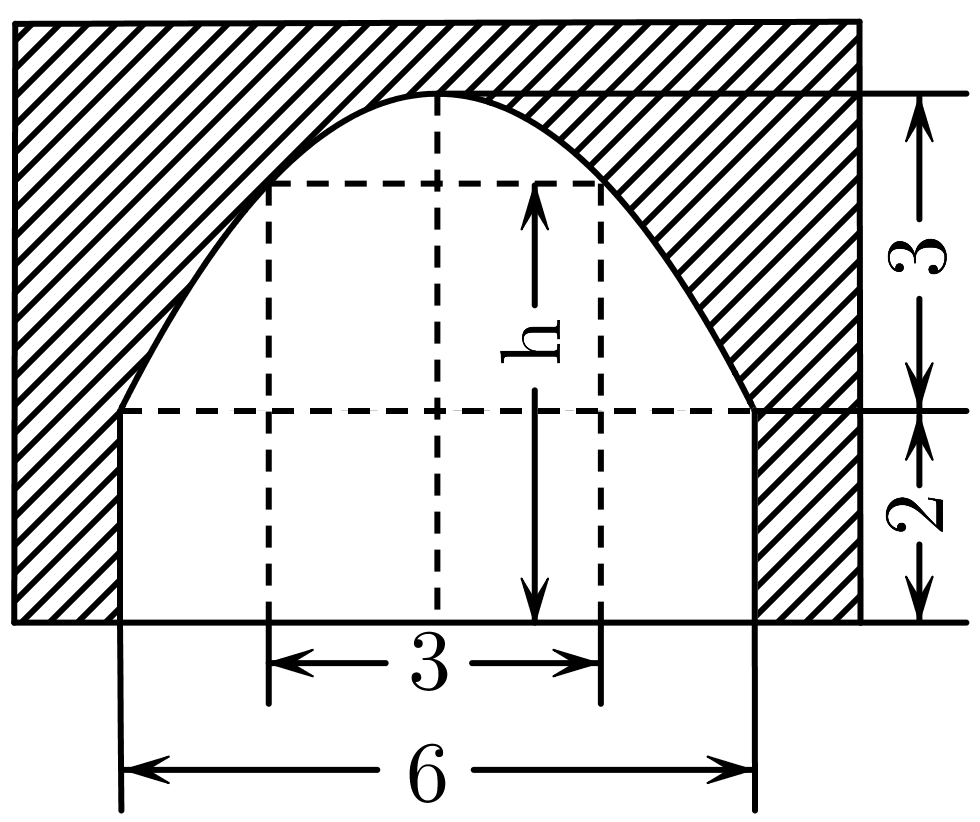
\includegraphics[width=40mm]{figs/15-16.png}}
\liubai[16mm]{解答书写区}

\begin{ansblock}[2章-练-课时15-16]
% ans:2章-练-课时15-16
\ansitem{16}{不能安全通过隧道。}
\ansnote{详解}{以抛物线顶点为原点、对称轴为\(y\)轴建系。由图：拱高3m、半宽3m，抛物线过\(A(3,-3)\)；矩形部分高2m、总高（顶点至地面）5m、地面\(y=-5\)。设\(x^{2}=-2py\)（\(p>0\)）：\(9=-2p\times (-3)\)，\(2p=3\)，方程\(x^{2}=-3y\)。\par\noindent 车居中：\(x=\pm 1.5\)处拱高\(y=-(1/3)\times 2.25=-0.75\)，净空\(=5-0.75=4.25\)(m)。\(4.25<4.5\)（车与集装箱总高），即使集装箱处于隧道正中，总高仍高于该处拱高，故不能安全通过。验算：\((\pm 1.5)^{2}=-3y\)得\(y=-0.75\)合；\(2p=3\)时准线\(y=3/4\)合。}
\end{ansblock}

% ---- 尾块（\tailfill 置 \end{multicols} 前；无参＝内容尾随框，每件恰 1 处） ----
\tailfill

\end{multicols}
\end{document}
